% Options for packages loaded elsewhere
\PassOptionsToPackage{unicode}{hyperref}
\PassOptionsToPackage{hyphens}{url}
%
\documentclass[
  11pt,
  letterpaper,
]{article}
\usepackage{amsmath,amssymb}
\usepackage{iftex}
\ifPDFTeX
  \usepackage[T1]{fontenc}
  \usepackage[utf8]{inputenc}
  \usepackage{textcomp} % provide euro and other symbols
\else % if luatex or xetex
  \usepackage{unicode-math} % this also loads fontspec
  \defaultfontfeatures{Scale=MatchLowercase}
  \defaultfontfeatures[\rmfamily]{Ligatures=TeX,Scale=1}
\fi
\usepackage{lmodern}
\ifPDFTeX\else
  % xetex/luatex font selection
\fi
% Use upquote if available, for straight quotes in verbatim environments
\IfFileExists{upquote.sty}{\usepackage{upquote}}{}
\IfFileExists{microtype.sty}{% use microtype if available
  \usepackage[]{microtype}
  \UseMicrotypeSet[protrusion]{basicmath} % disable protrusion for tt fonts
}{}
\makeatletter
\@ifundefined{KOMAClassName}{% if non-KOMA class
  \IfFileExists{parskip.sty}{%
    \usepackage{parskip}
  }{% else
    \setlength{\parindent}{0pt}
    \setlength{\parskip}{6pt plus 2pt minus 1pt}}
}{% if KOMA class
  \KOMAoptions{parskip=half}}
\makeatother
\usepackage{xcolor}
\usepackage[margin=1in]{geometry}
\usepackage{color}
\usepackage{fancyvrb}
\newcommand{\VerbBar}{|}
\newcommand{\VERB}{\Verb[commandchars=\\\{\}]}
\DefineVerbatimEnvironment{Highlighting}{Verbatim}{commandchars=\\\{\}}
% Add ',fontsize=\small' for more characters per line
\usepackage{framed}
\definecolor{shadecolor}{RGB}{248,248,248}
\newenvironment{Shaded}{\begin{snugshade}}{\end{snugshade}}
\newcommand{\AlertTok}[1]{\textcolor[rgb]{0.94,0.16,0.16}{#1}}
\newcommand{\AnnotationTok}[1]{\textcolor[rgb]{0.56,0.35,0.01}{\textbf{\textit{#1}}}}
\newcommand{\AttributeTok}[1]{\textcolor[rgb]{0.13,0.29,0.53}{#1}}
\newcommand{\BaseNTok}[1]{\textcolor[rgb]{0.00,0.00,0.81}{#1}}
\newcommand{\BuiltInTok}[1]{#1}
\newcommand{\CharTok}[1]{\textcolor[rgb]{0.31,0.60,0.02}{#1}}
\newcommand{\CommentTok}[1]{\textcolor[rgb]{0.56,0.35,0.01}{\textit{#1}}}
\newcommand{\CommentVarTok}[1]{\textcolor[rgb]{0.56,0.35,0.01}{\textbf{\textit{#1}}}}
\newcommand{\ConstantTok}[1]{\textcolor[rgb]{0.56,0.35,0.01}{#1}}
\newcommand{\ControlFlowTok}[1]{\textcolor[rgb]{0.13,0.29,0.53}{\textbf{#1}}}
\newcommand{\DataTypeTok}[1]{\textcolor[rgb]{0.13,0.29,0.53}{#1}}
\newcommand{\DecValTok}[1]{\textcolor[rgb]{0.00,0.00,0.81}{#1}}
\newcommand{\DocumentationTok}[1]{\textcolor[rgb]{0.56,0.35,0.01}{\textbf{\textit{#1}}}}
\newcommand{\ErrorTok}[1]{\textcolor[rgb]{0.64,0.00,0.00}{\textbf{#1}}}
\newcommand{\ExtensionTok}[1]{#1}
\newcommand{\FloatTok}[1]{\textcolor[rgb]{0.00,0.00,0.81}{#1}}
\newcommand{\FunctionTok}[1]{\textcolor[rgb]{0.13,0.29,0.53}{\textbf{#1}}}
\newcommand{\ImportTok}[1]{#1}
\newcommand{\InformationTok}[1]{\textcolor[rgb]{0.56,0.35,0.01}{\textbf{\textit{#1}}}}
\newcommand{\KeywordTok}[1]{\textcolor[rgb]{0.13,0.29,0.53}{\textbf{#1}}}
\newcommand{\NormalTok}[1]{#1}
\newcommand{\OperatorTok}[1]{\textcolor[rgb]{0.81,0.36,0.00}{\textbf{#1}}}
\newcommand{\OtherTok}[1]{\textcolor[rgb]{0.56,0.35,0.01}{#1}}
\newcommand{\PreprocessorTok}[1]{\textcolor[rgb]{0.56,0.35,0.01}{\textit{#1}}}
\newcommand{\RegionMarkerTok}[1]{#1}
\newcommand{\SpecialCharTok}[1]{\textcolor[rgb]{0.81,0.36,0.00}{\textbf{#1}}}
\newcommand{\SpecialStringTok}[1]{\textcolor[rgb]{0.31,0.60,0.02}{#1}}
\newcommand{\StringTok}[1]{\textcolor[rgb]{0.31,0.60,0.02}{#1}}
\newcommand{\VariableTok}[1]{\textcolor[rgb]{0.00,0.00,0.00}{#1}}
\newcommand{\VerbatimStringTok}[1]{\textcolor[rgb]{0.31,0.60,0.02}{#1}}
\newcommand{\WarningTok}[1]{\textcolor[rgb]{0.56,0.35,0.01}{\textbf{\textit{#1}}}}
\usepackage{graphicx}
\makeatletter
\def\maxwidth{\ifdim\Gin@nat@width>\linewidth\linewidth\else\Gin@nat@width\fi}
\def\maxheight{\ifdim\Gin@nat@height>\textheight\textheight\else\Gin@nat@height\fi}
\makeatother
% Scale images if necessary, so that they will not overflow the page
% margins by default, and it is still possible to overwrite the defaults
% using explicit options in \includegraphics[width, height, ...]{}
\setkeys{Gin}{width=\maxwidth,height=\maxheight,keepaspectratio}
% Set default figure placement to htbp
\makeatletter
\def\fps@figure{htbp}
\makeatother
\setlength{\emergencystretch}{3em} % prevent overfull lines
\providecommand{\tightlist}{%
  \setlength{\itemsep}{0pt}\setlength{\parskip}{0pt}}
\setcounter{secnumdepth}{5}
\newlength{\cslhangindent}
\setlength{\cslhangindent}{1.5em}
\newlength{\csllabelwidth}
\setlength{\csllabelwidth}{3em}
\newlength{\cslentryspacingunit} % times entry-spacing
\setlength{\cslentryspacingunit}{\parskip}
\newenvironment{CSLReferences}[2] % #1 hanging-ident, #2 entry spacing
 {% don't indent paragraphs
  \setlength{\parindent}{0pt}
  % turn on hanging indent if param 1 is 1
  \ifodd #1
  \let\oldpar\par
  \def\par{\hangindent=\cslhangindent\oldpar}
  \fi
  % set entry spacing
  \setlength{\parskip}{#2\cslentryspacingunit}
 }%
 {}
\usepackage{calc}
\newcommand{\CSLBlock}[1]{#1\hfill\break}
\newcommand{\CSLLeftMargin}[1]{\parbox[t]{\csllabelwidth}{#1}}
\newcommand{\CSLRightInline}[1]{\parbox[t]{\linewidth - \csllabelwidth}{#1}\break}
\newcommand{\CSLIndent}[1]{\hspace{\cslhangindent}#1}
\ifLuaTeX
\usepackage[bidi=basic]{babel}
\else
\usepackage[bidi=default]{babel}
\fi
\babelprovide[main,import]{spanish}
% get rid of language-specific shorthands (see #6817):
\let\LanguageShortHands\languageshorthands
\def\languageshorthands#1{}
\usepackage[utf8]{inputenc}
\usepackage{floatrow}
\floatsetup[figure]{capposition=top}
\usepackage{longtable}
\usepackage{array}
\usepackage{multirow}
\usepackage{booktabs}
\usepackage{longtable}
\usepackage{array}
\usepackage{multirow}
\usepackage{wrapfig}
\usepackage{float}
\usepackage{colortbl}
\usepackage{pdflscape}
\usepackage{tabu}
\usepackage{threeparttable}
\usepackage{threeparttablex}
\usepackage[normalem]{ulem}
\usepackage{makecell}
\usepackage{xcolor}
\ifLuaTeX
  \usepackage{selnolig}  % disable illegal ligatures
\fi
\IfFileExists{bookmark.sty}{\usepackage{bookmark}}{\usepackage{hyperref}}
\IfFileExists{xurl.sty}{\usepackage{xurl}}{} % add URL line breaks if available
\urlstyle{same}
\hypersetup{
  pdftitle={Problem Set 1: Predicting Income},
  pdfauthor={Gustavo Adolfo Castillo Álvarez (201812166),; Alexander Almeida Ramírez (202225165),; Jorge Luis Congacha Yunda (201920042) y; Jaime Orlando Buitrago González (200612390)},
  pdflang={es},
  hidelinks,
  pdfcreator={LaTeX via pandoc}}

\title{Problem Set 1: Predicting Income}
\usepackage{etoolbox}
\makeatletter
\providecommand{\subtitle}[1]{% add subtitle to \maketitle
  \apptocmd{\@title}{\par {\large #1 \par}}{}{}
}
\makeatother
\subtitle{Big Data y Machine Learning para Economía Aplicada}
\author{Gustavo Adolfo Castillo Álvarez (201812166), \and Alexander
Almeida Ramírez (202225165), \and Jorge Luis Congacha Yunda (201920042)
y \and Jaime Orlando Buitrago González (200612390)}
\date{03 de marzo de 2024}

\begin{document}
\maketitle

\hypertarget{introducciuxf3n}{%
\section{Introducción}\label{introducciuxf3n}}

Entre 1991 y 2019, el recaudo del impuesto a la renta aumentó en 7,1
puntos porcentuales (p.p.) dentro de la estructura tributaria de América
Latina y el Caribe, consolidándose como la segunda fuente de ingresos
(26,6\%), después de los impuestos generales sobre bienes y servicios
(CEPAL 2023). En contraste, para el último año, Colombia se encontró por
encima del promedio de sus pares regionales, pues el impuesto a la renta
representó el 32,3\% de su estructura tributaria; sin embargo, al
compararla carga la tributaria de este impuesto, Colombia está lejos del
grupo de países más desarrollados del cual hace parte, pues la renta
representa el 6,4\% del PIB, un valor lejano del promedio de la OCDE
(34\%).

Más aún para el 2019, el recaudo del impuesto de renta de las personas
correspondió a tan sólo al 1,3\% del PIB colombiano según la CEPAL
(2023). Este nivel de ingresos tributarios es considerablemente bajo y
se debe al complejo sistema tributario que permite mayores exensiones y
deducciones para quienes tienen ingresos más altos (Fergusson y
Hofstetter 2022), al mismo tiempo que las políticas, factores
psicológicos, coyunturas económicas y deficiencias administrativas
favorecen la evasión y elusión de este impuesto sobre los ingresos
(García, Parra, y Rueda 2021).

Cada reforma tributaria ha intentado mejorar los niveles de recaudo en
los últimos años, así mismo, los cambios administrativos en la DIAN
también han contribuido a este propósito, buscando un sistema tributario
más efciente y progresivo, ya que se cuenta con suficiente información y
evidencia para identificar sus principales problemas. No obstante, los
comportamientos de las personas, sobre todo aquellos asociados a
conductas delictivas (como la elusión y evasión), son más difíciles de
identificar ante su carácter ilegal y ético. Instrumentos como el
aprendizaje de máquinas (ML en adelante, por sus siglas en inglés)
pueden complementar y contribuir a aumentar el recaudo de los impuestos,
haciendo visible aquello que las personas buscan ocultar o esconder, es
decir, generando predicciones sobre los ingresos de las personas a
partir de características individuales, de los hogares, o incluso
territoriales.

Ha habido varios ejemplos del uso de técnicas de ML para abordar los
retos del recaudo de los impuestos. En Indonesia, a través de modelos
predictivos se identificaron potenciales pagos a las deudas por
impuestos a partir de los registros administrativos de la autoridad
fiscal de ese país (Febriminanto y Wasesa 2022); en Armenia, se pudieron
identificar posibles fraudes fiscales a partir de la información
reportada por los compradores y vendedores con herramientas de ML
(Baghdasaryan et~al. 2022); o en Brasil, Sao Paulo, se identificaron
potenciales pagadores, ingresos, el monto de los impuestos y multas a
partir de los registros administrativos de autoridad fiscal del
municipio (Ippolito y Garcia 2020).

Es por tanto, que en este Problem Set busca predecir el ingreso por hora
de los y las bogotanas mediante modelos que aprovechan las herramientas
del ML, haciendo uso de la principal encuesta de hogares colombiana. Más
específicamente, se utilizó la \emph{Medición de Pobreza Monetaria y
Desigualdad} (Sarmiento-Barbieri 2024) del 2018 para Bogotá, un módulo
de la \emph{Gran Encuesta Integrada de Hogares} (GEIH) del DANE, la cual
no sólo proporciona información sobre el mercado laboral, ingreso de las
personas, características socioeconómicas y territoriales, si no a su
vez representa una fuente de información confiable en la cual las
personas no tienen incentivos a reportar información falsa sobre su
ingreso, pues la encuesta es anónima y no tiene una finalidad
tributaria.

En este contexto, el presente documento \ldots(preview of the results an
main takeaways)

\hypertarget{datos}{%
\section{Datos}\label{datos}}

La GEIH es la principal y tal vez más importante encuesta de hogares con
la que cuenta Colombia actualmente. Mensualmente, el DANE recolecta
información sobre los ingresos y el mercado laboral de una muestra
representativa de la población colombiana, de tal manera, que cada mes
se obtienen datos sobre el ingreso y mercado laboral para el ámbito
nacional, y anualmente para 23 departamentos y Bogotá, sus capitales y
áreas metropolitanas, y otros dominios (rural y urbano) (DANE 2019). La
operación estadística tiene como resultado una base de datos anual de
aproximadamente 750 mil observaciones o personas, 230 mil hogares y 30
mil viviendas, la cual permite realizar cálculos y estimaciones sobre la
población colombiana.

Aunque la GEIH recolecta información sobre los ingresos y el mercado
laboral de la población, se realizan poco más de 150 preguntas a los
encuestados que capturan información demográfica, económica y social, de
tal manera que se expanden las posibilidades de la encuesta. Es así como
esta base de datos también permite caracterizar la migración,
micronegocios, la transición entre la educación y el trabajo, trabajo
infantil, tecnologías de la información y la pobreza monetaria (dentro
de los módulos más importantes). Este último módulo es importante para
el desarrollo del presente Problem Set, ya que el DANE agrega los
ingresos salariales y no salariales per cápita de las unidades de gasto
(hogares para simplificar), identificando las personas con ingresos
superiores e inferiores a las líneas de pobreza e indigencia definidas
en el Comité de Expertos
\footnote{Personas o representante de entidades nacionales o de cooperación internacional con la experticia técnica para orientar la operación estadística, cálculos y estimaciones de la pobreza monetaria}.
Es así como la GEIH es también la principal fuente de información para
calcular la incidencia, brecha y severidad de esta medición del
bienestar de la población.

La GEIH y su módulo sobre la \emph{Medición de Pobreza Monetaria y
Desigualdad} están disponibles al público en general a través de la
Archivo Nacional de Datos (ANDA) del DANE. Sus módulos anonimizados se
pueden descargar y unir para la investigación académica, la toma de
decisiones o cualquier propósito individual. En este caso, para el
Problem Set no se realizó el descargue de la página del DANE, sino se
realizó un \emph{web scraping} de la base de datos filtrada para Bogotá,
de la página web de Ignacio Sarmiento Barbieri (Sarmiento-Barbieri 2024)
como caso práctico de extracción de contenidos de una página web, con un
formato estructurado.

En la página web se encuentran 10 tablas en formato HTML, las cuales
contienen en total las 32.177 observaciones que componen la muestra de
personas para Bogotá de la GEIH para 2018, con 179 variables (21
variables adicionales a las presentes en la base de datos del ANDA). Al
encontrarse en un formato estructurado (tabla HTML), se realizó el
\emph{web scrpaing} haciendo uso del paquete \texttt{RSelenium} de
\texttt{RStudio}, con el cual se automatiza la consulta de cada una de
los 10 hipervínculos de la página web, se identifica la tabla en HTML,
se almacena y posteriormente se consolida una sola base de datos con las
características anteriormente mencionadas.

Como complemento, se descargaron y unieron las bases de datos de la GEIH
de 2018 (DANE 2022), de tal manera que se obtuviesen variables
complementarias para el desarrollo del Problem Set. Más específicamente,
los años de escolaridad, la rama de actividad
\footnote{Código a dos dígitos de la Clasificación Industrial Internacional Uniforme de todas las actividades Económicas (CIIU).}
y la pregunta sobre la posición ocupacional de las personas ocupadas. De
esta manera, se obtuvieron variables complementarias como escolaridad
como variable continua, experiencia laboral
\footnote{ Variable *proxy* construida como  Edad-Años de escolaridad-Años de ingreso al sistema educativo (6 años)},
sector económico y posición ocupacional.

Finalmente, se filtró la base de datos con las personas mayores de 18
años, quedando en total 16.542 observaciones o personas para el
desarrollo del Problem Set. De esta manera, a continuación se presentan
las estadísticas descriptivas de las variables utilizadas en los
siguientes puntos.

\begin{table}[H] \centering 
  \caption{Estadísticas descriptivas. Variables continuas} 
  \label{} 
\begin{tabular}{@{\extracolsep{5pt}}lcccccc} 
\\[-1.8ex]\hline 
\hline \\[-1.8ex] 
Statistic & \multicolumn{1}{c}{N} & \multicolumn{1}{c}{Mean} & \multicolumn{1}{c}{St. Dev.} & \multicolumn{1}{c}{Min} & \multicolumn{1}{c}{Median} & \multicolumn{1}{c}{Max} \\ 
\hline \\[-1.8ex] 
Ingreso laboral (miles) & 9,892 & 1,745.42 & 2,403.44 & 20.00 & 1,032.56 & 60,100.00 \\ 
Experiencia laboral & 16,541 & 22.01 & 15.16 & $-$7 & 19 & 81 \\ 
Edad & 16,542 & 39.44 & 13.48 & 18 & 38 & 94 \\ 
Años de escolaridad & 16,541 & 11.43 & 4.34 & 0 & 11 & 26 \\ 
\hline \\[-1.8ex] 
\end{tabular} 
\end{table}

\begin{table}[H]

\begin{center}
\begin{threeparttable}

\caption{\label{tab:descriptive_categorical}Frecuencias variables categóricas}

\begin{tabular}{llr}
\toprule
Variable & \multicolumn{1}{c}{N} & \multicolumn{1}{c}{\%}\\
\midrule
Posición ocupacional &  & \\
\ \ \ Obrero, empleado particular & 9342 & 56.47\\
\ \ \ Obrero, empleado del gobierno & 632 & 3.82\\
\ \ \ Empleado doméstico & 578 & 3.49\\
\ \ \ Trabajador por cuenta propia & 5106 & 30.87\\
\ \ \ Patrón o empleador & 626 & 3.78\\
\ \ \ Trabajador familiar sin remuneración & 207 & 1.25\\
\ \ \ Trabajador sin remuneración en empresas de otros hogares & 41 & 0.25\\
\ \ \ Jornalero o Peón & 1 & 0.01\\
\ \ \ Otro & 9 & 0.05\\
Sector &  & \\
\ \ \ Agricultura, ganadería, caza, silvicultura y pesca & 106 & 0.64\\
\ \ \ Explotación de Minas y Canteras & 50 & 0.30\\
\ \ \ Industria manufacturera & 2470 & 14.93\\
\ \ \ Suministro de Electricidad Gas y Agua & 77 & 0.47\\
\ \ \ Construcción & 881 & 5.33\\
\ \ \ Comercio, hoteles y restaurantes & 4581 & 27.69\\
\ \ \ Transporte, almacenamiento y comunicaciones & 1484 & 8.97\\
\ \ \ Intermediación financiera & 496 & 3.00\\
\ \ \ Actividades inmobiliarias, empresariales y de alquiler & 2534 & 15.32\\
\ \ \ Servicios comunales, sociales y personales & 3863 & 23.35\\
Sexo &  & \\
\ \ \ Hombre & 8767 & 53.00\\
\ \ \ Mujer & 7775 & 47.00\\
\bottomrule
\end{tabular}

\end{threeparttable}
\end{center}

\end{table}

De las 32177 observaciones, se puede observar la tasa de valores
perdidos de las variables de interés:

\hypertarget{modelo}{%
\section{Modelo}\label{modelo}}

El modelo

\hypertarget{perfiles-de-salario-por-edad}{%
\section{Perfiles de salario por
edad}\label{perfiles-de-salario-por-edad}}

Para empezar a caracterizar los determinantes de los salarios, vamos a
realizar una estimación que explore la relación entre ingresos y edad.
Existe literatura que encuentra que los salarios tienden a seguir una
distribución de u invertida, en la que el máximo salario se obtiene a
los 50 años. A partir de esta edad, comienza a observarse disminuciones
significativas en los salarios (Skirbekk, 2004). Entre las posibles
explicaciones de este suceso está relacionado con la productividad. Las
personas cuando comienzan su vida laboral tienden a tener menos
experiencia y habilidades especializadas, por lo que sus salarios son
más bajos al inicio de sus carreras. A partir de algún momento de la
edad adulta, las capacidades cognitivas y físicas empiezan a disminuir.

Estudiar esta relación es importante en la medida en que es importante
determinar los salarios por edad con el fin de realizar un perfilamiento
de los ingresos por grupos de edad. Por tal motivo, se plantea estimar
la siguiente regresión por medio de Mínimos Cuadrados Ordinarios para
analizar la relación entre salarios y edad:

\[
log(salario_i)=\beta_0{}+\beta_1 Edad +\beta_2  Edad^2 +u_i
\] Dónde \(Salario_i\) corresponde a los ingresos asalariados +
independientes total nominal por hora. Se realiza la transformación
logarítmica con el fin de facilitar la interpretación de los
coeficientes de la regresión. La \(Edad\) y la \(Edad^2\) corresponden a
la edad para cada individuo \(i\). La inclusión del término cuadrático
permite modelar la relación en u invertida entre salarios y la edad y el
término \(u_i\) corresponde al término error idiosincrático, que
representa las variables que no están en nuestro modelo y que explican
los salarios.

Sin embargo, debido a que este modelo tiene un posible problema de
endogeneidad (en la medida en la que la edad está correlacionada con
otras variables como la educación y la experiencia), decidimos hacer un
ejercicio adicional, en el que se incluyen controles con el fin de
mejorar la inferencia causal. Las variables explicativas que agregamos
son: horas trabajadas a la semana, el sexo de los individuos, ocupación,
tipo de ocupación y su máximo nivel educativo.

En la tabla tal se pueden observar los resultados de las estimaciones.
La columna 1 muestra los resultados de la estimación sin controles,
mientras que la columna 2 presenta la regresión con controles. Se puede
observar que, en promedio, un aumento de un año en la edad está asociado
con un incremento en el salario del 5.5\% (modelo sin controles) y del
6.4\% (modelo con controles). Estos resultados muestran que nuestra
especificación es robusta en la medida en que los resultados no
presentan un gran cambio en magnitud. Sin embargo, debido a que estamos
estimando una relación no lineal entre la edad y el salario, la
interpretación no es tan intuitivamente porque debemos tener en cuenta
el \(\beta_2\) de la regresión.


% Table created by stargazer v.5.2.3 by Marek Hlavac, Social Policy Institute. E-mail: marek.hlavac at gmail.com
% Date and time: dom., mar. 03, 2024 - 9:54:46 p. m.
% Requires LaTeX packages: dcolumn 
\begin{table}[!htbp] \centering 
  \caption{Resultados de la regresion} 
  \label{} 
\begin{tabular}{@{\extracolsep{5pt}}lD{.}{.}{-3} D{.}{.}{-3} } 
\\[-1.8ex]\hline 
\hline \\[-1.8ex] 
 & \multicolumn{2}{c}{Logaritmo del salario} \\ 
\cline{2-3} 
 & \multicolumn{1}{c}{Con controles} & \multicolumn{1}{c}{Sin controles} \\ 
\\[-1.8ex] & \multicolumn{1}{c}{(1)} & \multicolumn{1}{c}{(2)}\\ 
\hline \\[-1.8ex] 
 Edad & 0.067^{***} & 0.147^{***} \\ 
  & (0.004) & (0.003) \\ 
  & & \\ 
 Edad al cuadrado & -0.001^{***} & -0.0004^{***} \\ 
  & (0.00004) & (0.00003) \\ 
  & & \\ 
\hline \\[-1.8ex] 
Observaciones & \multicolumn{1}{c}{9,891} & \multicolumn{1}{c}{9,891} \\ 
R$^{2}$ & \multicolumn{1}{c}{0.044} & \multicolumn{1}{c}{0.476} \\ 
Adjusted R$^{2}$ & \multicolumn{1}{c}{0.044} & \multicolumn{1}{c}{0.475} \\ 
\hline 
\hline \\[-1.8ex] 
\textit{Note:}  & \multicolumn{2}{r}{$^{*}$p$<$0.1; $^{**}$p$<$0.05; $^{***}$p$<$0.01} \\ 
\end{tabular} 
\end{table} 


En cuanto al coeficiente de la variable edad al cuadrado no cambia para
ninguno de los modelos. Lo más importante de este coeficiente es su
signo negativo. Esto indica que hay una relación cóncava entre el
salario y la edad, resultado esperado por la teoría. Para poder
interpretar correctamente el coeficiente de la edad, debemos derivar con
respecto a la edad:

\[
\frac{\partial log(salario)}{\partial Edad} =\beta_1  +2 \beta_2 Edad
\]

Encontramos que la interpretación depende del nivel de edad que se
analiza. Para realizar el análisis, estimamos la edad promedio de la
base de datos (38 años). Encontramos que, para un individuo con una edad
de 38 años, un año adicional está asociado con un aumento en el salario
del 1.7\%. Para la interpretación del \(\beta_{0}\), sería como el
logaritmo del salario promedio cuando las personas tienen 0 años de
edad. Aunque esta puede tener una intepretación poco intuitiva, debido a
que nuestra muestra está acotada a personas de 18 años, se interpretaría
como el salario promedio cuando los individuos inician su vida laboral.

En cuanto a la interpretación del coeficiente de determinación(r2) nos
indica que, aproximadamente, el 2.3\% de la variación del logaritmo del
salario es explicada por la edad. Aunque este r2 puede ser bajo, es
explicado porque existen muchos más factores que explican el salario.
Por esto, cuando vemos el r2 del modelo con controles, encontramos que
ell r2 se incrementa hasta aproximadamente el 34\%. Sin embargo, estas
variables son significativas a un nivel de significancia del 5\%, lo que
indica que la edad es un determinante del salario.

Ahora, vamos a encontrar la edad en la que empiezan a disminuir los
ingresos de las personas. Para hacerlo, debemos encontrar el punto
máximo de la función que estimamos e igualar a cero. Haciendo el
procedimiento, obtenemos que esta edad máxima está dada por:
\(edad_{max}=-\beta_1/2\beta_2\). Reemplazando estos valores en esta
ecuación, encontramos que la edad máxima en la que se alcanza el máximo
rendimiento de los salarios se alcanzan a los 49.65 años. Este valor es
esperado según la literatura (citar literatura).

Para analizar esto mejor, en la figura tal se puede observar la relación
entre la edad y los salarios. En la primera mitad de la gráfica, se
puede observar que aumentan los salarios a medida que aumenta la edad.
Esto es explicado debido a que las personas cuentan con cada vez más
experiencia y habilidades, hasta llegar a su máximo ingreso a los 49.65
años, en los que los incrementos comienzan a disminuir hasta niveles más
bajos que los incrementos al comienzo de su vida laboral. Como se
discutió al principio de la sección, puede deberse a múltiples razaones
como un retraso en el aprendizaje de nuevas habilidades por la reducción
de capacidad cognitiva, lo que implica tener más dificultad para
ascender o encontrar empleos con mayores ingresos.

En la fráfica anterior también se pueden observar los intervalos de
confianza al nivel de confianza del 95\%. Estos intervalos fueron
construidos con errores estándar boortraps, en la que se relizaron 1000
repeticiones de la regresión sin controles con un resampleo de la
muestra para cada repetición. Es importante notar que estos intervalos
crecen a medida que la edad aumeta, esto puede deberse a que existe
mucha heterogeneidad de salarios en las personas con edades mayores,
porque, por ejemplo, existen personas con salarios muy altos (con
posiciones gerenciales, por ejemplo) mientras que otras personas
continuaron con puestos relativamente bajos o que están cerca de la edad
de jubilación, por lo que sus salarios disminuirían.

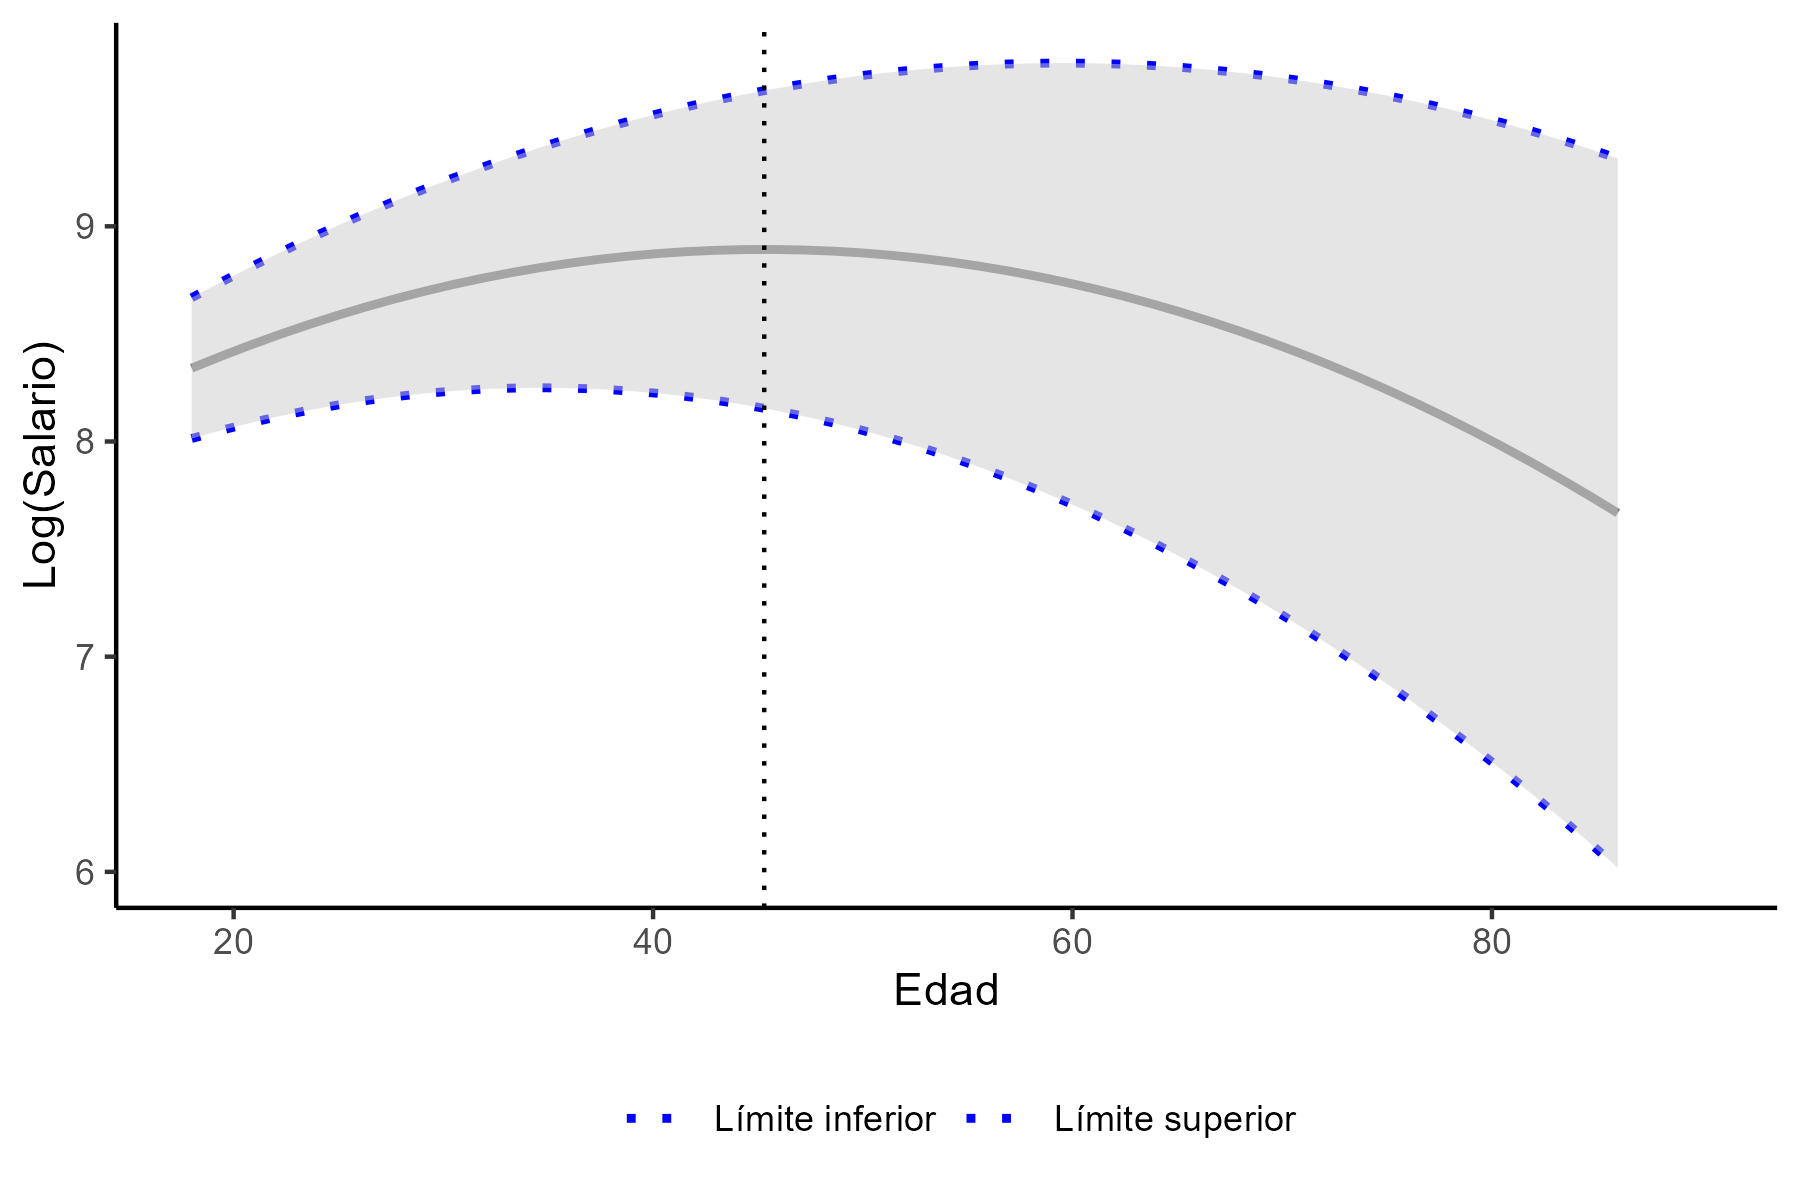
\includegraphics[width=25in]{../views/age_earnings_plot}

\hypertarget{brechas-de-ingreso-por-sexo}{%
\section{Brechas de ingreso por
sexo}\label{brechas-de-ingreso-por-sexo}}

\begin{enumerate}
\def\labelenumi{\alph{enumi})}
\tightlist
\item
  En esta sesión se intenta predecir la brecha salarial del logaritmo
  del ingreso entre hombres y mujeres. Para ello, comenzamos estimando
  el modelo más sencillo de todos, es decir, el modelo univariado:
\end{enumerate}

\begin{equation}
\ln (w) = \beta_1 + \beta_2 Mujer+u
  \label{gap0}
\end{equation}

Los resultados de la regresión muestran que en promedio, el salario de
una mujer es 4,37\% menor en comparación con el salario de un
hombre.Esto con un nivel de significacion del 5\% y con un error
estándar de 0.733.

\begin{table}[H] \centering 
  \caption{Estimando brecha de género} 
  \label{} 
\begin{tabular}{@{\extracolsep{5pt}}lcc} 
\\[-1.8ex]\hline 
\hline \\[-1.8ex] 
 & \multicolumn{2}{c}{\textit{Dependent variable:}} \\ 
\cline{2-3} 
\\[-1.8ex] & \multicolumn{2}{c}{Ln Salario} \\ 
\\[-1.8ex] & (1) & (2)\\ 
\hline \\[-1.8ex] 
 age &  & 0.012$^{***}$ \\ 
  &  & (0.001) \\ 
  & & \\ 
 womanMujer & $-$0.144$^{***}$ & $-$0.124$^{***}$ \\ 
  & (0.016) & (0.014) \\ 
  & & \\ 
 relab &  & 0.126$^{***}$ \\ 
  &  & (0.020) \\ 
  & & \\ 
 Constant & 14.076$^{***}$ & 13.898$^{***}$ \\ 
  & (0.011) & (0.192) \\ 
  & & \\ 
\hline \\[-1.8ex] 
Observations & 9,964 & 9,963 \\ 
R$^{2}$ & 0.009 & 0.453 \\ 
Adjusted R$^{2}$ & 0.008 & 0.448 \\ 
Residual Std. Error & 0.775 (df = 9962) & 0.579 (df = 9876) \\ 
F Statistic & 86.083$^{***}$ (df = 1; 9962) & 94.912$^{***}$ (df = 86; 9876) \\ 
\hline 
\hline \\[-1.8ex] 
\textit{Note:}  & \multicolumn{2}{r}{$^{*}$p$<$0.1; $^{**}$p$<$0.05; $^{***}$p$<$0.01} \\ 
 & \multicolumn{2}{r}{Controles: oficio, maxEduclevel} \\ 
\end{tabular} 
\end{table}

El coeficiente \(\beta_2<0\) indica que las mujeres, en promedio y
ceteris praibus, reciben un salario mensual NA menos ingresos que los
hombres.

\begin{enumerate}
\def\labelenumi{\Alph{enumi})}
\setcounter{enumi}{1}
\tightlist
\item
  Para mejorar la estimación anterior se corrió un modelo condicional en
  donde se incluye controles como características similiares de
  trabajadores y puestos de trabajo. Para ello se recurrio al uso de FWL
  y FWL con boostrap.
\end{enumerate}

\hypertarget{estimaciuxf3n-fwl}{%
\subsection{Estimación FWL:}\label{estimaciuxf3n-fwl}}

En la primera etapa, \emph{partialling-out}, ejecutamos dos regresiones.
Definimos nuestra variable de interés a la variable dicotómica de
\(Mujer\). Con esto corremos la primera regresión para estimar
\texttt{woman\textasciitilde{}x1+x2+...}, donde las \texttt{xi} son
todas aquellas variables de control usadas para corregir el potencial
sesgo de variable omitida. Posteriormente nos quedamos con los
residuales \texttt{woman\_res}, y ejecutamos una segunda regresión en la
que estimemos \texttt{log\_wage\textasciitilde{}x1+x2...}, y guardamos
estos residuales, \texttt{log\_wage\_res}.

Finalmente ejecutamos la segunda regresión univariada
\texttt{log\_wage\_res\textasciitilde{}woman\_res} y obtenemos el mismo
coeficiente del modelo original con controles.Los resultados dejan ver
que una vez incorporado controles a la regresión de gap, se tiene que el
salario de las mujeres es en promedio menor en 16.5\% respecto al
salario del hombre, ceteris paribus.

\hypertarget{estimaciuxf3n-fwl-con-boostrap}{%
\subsection{Estimación FWL con
boostrap:}\label{estimaciuxf3n-fwl-con-boostrap}}

Por otra parte, estimando el modelo con FWL y boostrap se puede apreciar
que el valor del gap es el mismo del modelo anterior, es decir, el gap
es del 16.54\%. Con este obtenemos el mismo valor de gap, sin embargo el
valor del error estandar para la estimación con FWL y Boostra es es
menor, siendo est de 0.0122. Esta diferencia se da debido aque FWL asume
que su modelo es homcedastico, lo cual no es verdadero.

\begin{enumerate}
\def\labelenumi{\alph{enumi})}
\setcounter{enumi}{2}
\item
  \begin{figure}
  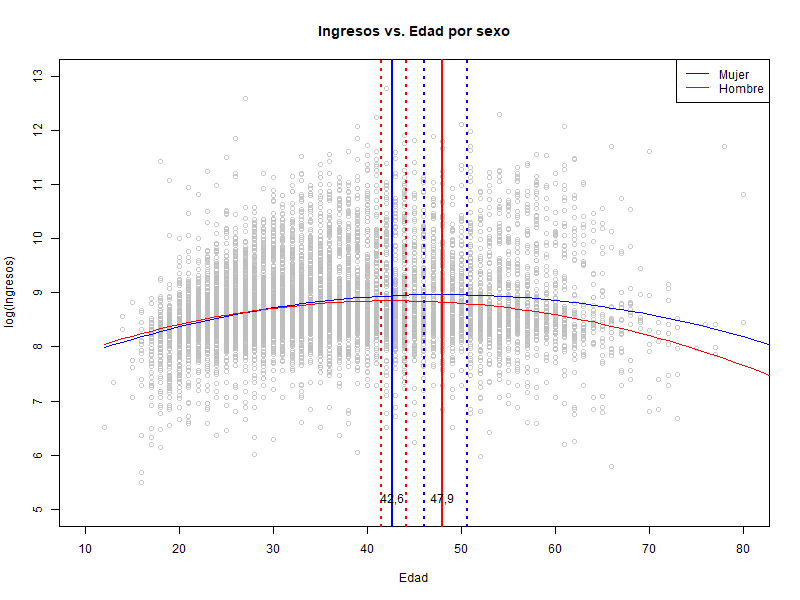
\includegraphics[width=0.7\linewidth]{../views/earnings_peak_ages} \caption{Perfil de ingresos vs edad por sexo}\label{fig:unnamed-chunk-2}
  \end{figure}
  \begin{center}\footnotesize{Fuente: Cálculos propios a partir de @geih}\end{center}
\end{enumerate}

El calculo de los picos de los salarios para cada sexo se realizó a
partir de dos regresiones

\hypertarget{predicciuxf3n-de-salarios}{%
\section{Predicción de salarios}\label{predicciuxf3n-de-salarios}}

\hypertarget{referencias-bibliogruxe1ficas}{%
\section{Referencias
bibliográficas}\label{referencias-bibliogruxe1ficas}}

\hypertarget{refs}{}
\begin{CSLReferences}{1}{0}
\leavevmode\vadjust pre{\hypertarget{ref-bdsn}{}}%
Baghdasaryan, V., H. Davtyan, A. Sarikyan, y Z. Navasardyan. 2022.
{«Improving Tax Audit Efficiency Using Machine Learning: The Role of
Taxpayer's Network Data in Fraud Detection»}. \emph{Applied Artificial
Intelligence} 36 (1): 2012002.
\url{https://doi.org/10.1080/08839514.2021.2012002}.

\leavevmode\vadjust pre{\hypertarget{ref-cepal}{}}%
CEPAL. 2023. \emph{Panorama fiscal de América Latina y el Caribe 2023}.
CEPAL.

\leavevmode\vadjust pre{\hypertarget{ref-dane18}{}}%
DANE. 2019. {«Medición de Pobreza Monetaria y Desigualdad 2018»}.
{[}Base de
datos{]}.\path{https://microdatos.dane.gov.co/index.php/catalog/608}

\leavevmode\vadjust pre{\hypertarget{ref-dane}{}}%
DANE. 2022. {«Gran Encuesta Integrada de Hogares 2018. Empalmada»}.
{[}Base de
datos{]}.\path{https://microdatos.dane.gov.co/index.php/catalog/758}

\leavevmode\vadjust pre{\hypertarget{ref-fw}{}}%
Febriminanto, R., y M Wasesa. 2022. {«Machine Learning Analytics for
Predicting Tax Revenue Potential»}. \emph{Indonesian Treasury Review} 7
(3): 193-205.

\leavevmode\vadjust pre{\hypertarget{ref-undp}{}}%
Fergusson, L., y M. Hofstetter. 2022. {«The Colombian tax system: A
diagnostic review and proposals for reform»}. UNDP.

\leavevmode\vadjust pre{\hypertarget{ref-ex}{}}%
García, M., O. Parra, y F. Rueda. 2021. {«Features of tax structure and
tax evasion in Colombia»}. \emph{Apuntes Contables}, n.º 28: 17-40.

\leavevmode\vadjust pre{\hypertarget{ref-ig}{}}%
Ippolito, A., y A. Garcia. 2020. {«Tax Crime Prediction with Machine
Learning: A Case Study in the Municipality of Sao Paulo»}. \emph{ICEIS
2020} 1: 452-59.

\leavevmode\vadjust pre{\hypertarget{ref-geih}{}}%
Sarmiento-Barbieri, I. 2024. {«Problem Set 1. BDML»}. {[}Base de
datos{]}.\path{https://ignaciomsarmiento.github.io/GEIH2018_sample/}

\end{CSLReferences}

\hypertarget{ejemplos}{%
\section{Ejemplos}\label{ejemplos}}

Para incrustar código y resultados de la consola

\begin{Shaded}
\begin{Highlighting}[]
\FunctionTok{summary}\NormalTok{(cars)}
\end{Highlighting}
\end{Shaded}

\begin{verbatim}
##      speed           dist       
##  Min.   : 4.0   Min.   :  2.00  
##  1st Qu.:12.0   1st Qu.: 26.00  
##  Median :15.0   Median : 36.00  
##  Mean   :15.4   Mean   : 42.98  
##  3rd Qu.:19.0   3rd Qu.: 56.00  
##  Max.   :25.0   Max.   :120.00
\end{verbatim}

Para incluir ecuaciones

\[
w=f(X)+u
\]

Para incluir gráficas

\begin{figure}

{\centering \includegraphics{Document_files/figure-latex/unnamed-chunk-3-1} 

}

\caption{Título de la gráfica}\label{fig:unnamed-chunk-3}
\end{figure}
\begin{center}\footnotesize{Fuente: Cálculos propios a partir de @geih}\end{center}

\end{document}
